\section{Introduction}
\subsection{Statement of the Problem}
Nowadays,  traffic capacity is limited by the number of lanes of roads in many regions of United States,  hence self-driving and cooperating cars ha been proposed as a solution to increase capacity of highways without increasing number of lanes or roads.  However,  the cooperation between self-driving cars as well as the interaction between self-driving and non-self-driving vehicles are still not well understood.


The Governor of the state of Washington has asked for analysis of the effects of allowing self-driving and cooperating cars on Interstates5,  90,  405 and State Route520,  also give how do the effects change when the percentage of self-driving cars alter.  In order to meet the demands,  we improve.  .  .  which is based on Cellular Automaton in order to describe the changing situation of traffic flow in the transportation network.

\subsection{Our work}
%Two major problems are discussed in this paper,   which are:
%\begin{itemize}
%    \item Doing the first thing.
%    \item Doing the second thing.
%\end{itemize}


\section{Detailed Definitions and Assumptions}
%A literatrue\cite{1} say something about this problem .  .  .
\subsection{Detailed Definitions}
The detailed definitions are listed as follows:
\begin{table}[h]
    \begin{center}
        \caption{Detailed Definitions}
        \hspace{1cm}
        \begin{tabular}{p{60pt}p{350pt}}
            \toprule
            \textbf{Denotation}&\textbf{Definition}\\
            \midrule
            $L$&The length of road\\
            ${\delta _x}$&The length of road each cellular\\
            $V$&The velocity of each vehicle\\
            ${v_{\max }}$&The maximum velocity of vehicles\\
            $t$&The moment\\
            $n$&The n-th car\\
            ${x_n}(t)$&The displacement of the n-th car in t moment\\
            ${v_n}(t)$&The velocity of the n-th car in t moment\\
            $Ga{p_n}(t)$&The actual gap between the n-th car and the neighbor foregoing car\\
            $Ga{p_{safe,n}}(t)$&The safe gap between the n-th car and the neighbor foregoing car\\
            $Ga{p_{ni}}(t)$&The gap between the n-th car and the neighbor foregoing car on the next  i-th lane in t moment\\
            $Ga{p_{ni,back}}(t)$&The gap between the n-th car and the neighbor posterior car on the next  i-th lane in t moment\\
            ${P_{n,change}}(t)$&The probability that the n-th car change lines when the situation is satisfied to change lines\\
            ${v_{safe,n}}(t)$&The velocity that the n-th car keep the safe gap from the neighbor foregoing car in t moment\\
            ${a_n}(t)$&The acceleration of the n-th car in t moment\\
            $P$&The retardation probability of vehicle velocity\\
            ${P_0}$&The initial retardation probability of vehicle velocity\\
            $P(t)$&The retardation probability of vehicle velocity in t moment\\
            $\alpha $&The memory parameter towards the last time randomization retardation probability of drivers\\
            $\beta $&The probability that driver forget nonoccurrence of randomization retardation in the last moment totally\\
            $\gamma $&The probability that the car go straight\\
            $\theta $&The traffic flow of the road section\\
            $J$&The traffic flow\\
            $\rho $&The response parameter to describe the response speed of drivers\\
            \bottomrule
        \end{tabular}\label{Ntt}
    \end{center}
\end{table}\newpage

\subsection{Assumptions}
\begin{enumerate}[\bfseries 1.  ]
 \item For conceptual clarification,   this statement categorizes the operations of vehicle into 5 levels,   from fully-manual (0) to fully-automated driving (4),   depending on the level of automation.  But in order to simplify the model,  We divide the categories into two types,  one is fully-automated driving,  and the other is manual driving.
 \item The limitation of velocity on the roads are assumed to be the same.   In practice,   there might be slight difference.
\end{enumerate}

\section{NS-LSMS Model}
In order to describe traffic capacity,  we adopt NS method which is proposed by Nagel and Schreckenberg as our basic model.  After some improvements about the model conducted by scholars,  the current NS method can describe the non-linear phenomena such as metastable state and hysteresis in single lane traffic environment.

Based on the available model mentioned above,  to consider the situation of transportation network in Washington,  we take lanes traffic environment,  sections traffic environment and experience into account.  To meet the demand of the Governor of Washington,  we build the NS-LSMS Model to  express the traffic capacity in Washington that allows self-driving and cooperating cars on the roads then propose a optimum proposal.

\subsection{Part 1 :Basic NS Model}
We divide a L length road into several discrete cellulars which length is .  Each cellular has two states denoted S that ranges from 0 to 1.  Therein,  0 means there is a car when 1 means no car.  We use t to denote the velocity of each vehicle,  for it values as 0,  1,  2...,  ${v_{\max }}$ .  We set the time span of the simulation iteration is 1s.  The rules of NS model are listed as follows:
\begin{figure}[htbp]
    \small
    \centering
    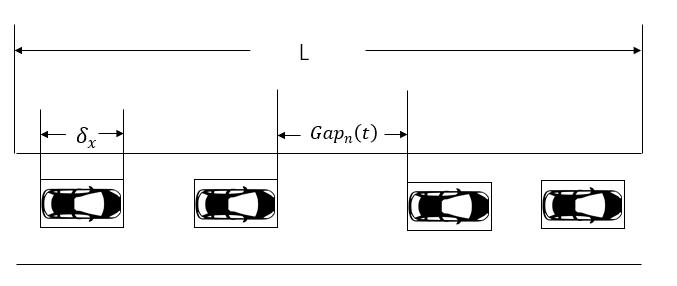
\includegraphics[width=12cm]{2.jpg}\\
    \caption{The rules of NS model}
        \label{Ntt}
\end{figure}


{\bf Acceleration rule: }When the actual gap between the n-th car and the neighbor foregoing car farther than the safe gap,  that is $Ga{p_n}(t) > Ga{p_{safe,  n}}(t)$ ,   the posterior car can accelerate with ${a_n}(t)$ acceleration  so as to run faster.  During the driving process,  the vehicle velocity ${v_{\max }}$ must not exceed the maximum velocity  in this lane also be less than the safe gap $Ga{p_{safe,  n}}(t)$ distance from the neighbor foregoing car.  Then we have:
\begin{equation}
{v_n}(t + 1) = \min ({v_n}(t) + {a_n}(t),  {v_{\max }},  Ga{p_n}(t))
\end{equation}


{\bf Randomization retardation rule: }Because the uncertainty factors in the road environments can cause the randomly change of vehicle velocity,  we premise randomization retardation rule then deceleration rule and employ $p$ ,   ${a_n}(t)$ to denote randomization retardation probability and randomization deceleration.  Then we have randomization retardation rule:
\begin{equation}
{v_n}(t + 1) = \max ({v_n}(t) - {a_n}(t),  0)
\end{equation}

{\bf Deceleration rule: }When the actual gap between the n-th car and the neighbor foregoing car closer than the safe gap,  that is $Ga{p_n}(t) < Ga{p_{safe,  n}}(t)$ .  In this situation,  the posterior car should decelerate to ensure the traffic safety.  We obtain the deceleration rule:
\begin{equation}
{v_n}(t + 1) = \min ({v_n}(t),  {v_{safe,  n}}(t))
\end{equation}


{\bf Location update rule: }After the update of vehicle velocity,  we update the vehicle location subject to following rule.  When the displacement farther than the length of the road section $L$ ,  we remove this car and decrease the total vehicle number $N$ for it has left this section.  Then we write the formulas to update the vehicle location and remove the car as follows:
\begin{equation}
{x_n}(t + 1) = {x_n}(t) + {v_n}(t + 1)
\end{equation}


When ${x_n}(t + 1) \le L$ ,   $N$ is invariant;


When ${x_n}(t + 1) > L$ ,  We obtain:
\begin{equation}
N=N-1
\end{equation}


The above-mentioned variables${v_{safe,  n}}(t)$,  $Ga{p_{safe,  n}}(t)$,  $Ga{p_n}(t)$can be calculated as follow:
\begin{equation}
Ga{p_n}(t) = {x_{n + 1}}(t) - {x_n}(t)
\end{equation}
\begin{equation}
Ga{p_{safe,  n}}(t) = {{{v_n}{{(t)}^2}} \over {2{a_n}(t)}} - {{{v_{n + 1}}{{(t)}^2}} \over {2{a_{n + 1}}(t)}}
\end{equation}


When $Ga{p_n}(t) > Ga{p_{safe,  n}}(t)$ ,  we have:
\begin{equation}
{v_{safe,  n}}(t) = {(2{a_n}(t)Ga{p_n}(t) - {v_n}{(t)^2})^{{1 \over 2}}}
\end{equation}


Or when $Ga{p_n}(t) < Ga{p_{safe,  n}}(t)$ ,  then:
\begin{equation}
{v_{safe,  n}}(t) = \max ({(2{a_n}(t)Ga{p_n}(t) - {v_n}{(t)^2})^{{1 \over 2}}},  0)
\end{equation}


\subsection{Part 2 :Lanes traffic environment}
Aiming at the supplied data,  there are 2,   3,   4 and5 lanes types on lanes traffic environment in the single side.  Therefore,  we add 4 rules to describe the situation of changing lanes .  For It is impossible for all vehicles to change lanes at all times logically,  we divide changing lanes into 2 processes.  One is to determine whether the situation is meeting changing lanes demand,  the other is to determine whether the car will execute changing lanes.  Then we have:
\begin{equation}
Ga{p_n}(t) < \delta
\end{equation}
\begin{equation}
Ga{p_{ni}}(t) > m\delta
\end{equation}
\begin{equation}
Ga{p_{ni,  back}}(t) > n\delta
\end{equation}
\begin{equation}
rand() < {P_{n,  change}}(t)
\end{equation}


The location changing rule is:
\begin{equation}
{x_n}(t) = {x_{n,  change}}(t)
\end{equation}


Therein,  we neglect the rule (10) when the car is in passing lane on asymmetrical lanes condition.  That is,    no matter if the front is free,   the car should return back to traffic lane instead of running in passing lane if there is enough free space in traffic lane.  The mentioned two lanes are the left-most lane of the Interstate,  car pool lane,  and the called "dead lane" used to turn left.


\subsection{Part 3 :Sections traffic environment}
Aiming at the supplied map,  the phenomenon of changing road sections may occur at different crossing entrances.  We simply divide the vehicles behaviors at the intersection into two situations:running straight or turning.


At the intersection, we do not take the impact of traffic lights on vehicles into consideration. For the running straight vehicles,  they keep the original speed to run straight. For the turning vehicles, we do not strictly differentiate between turning left or right in order to simplify the problem. We set the turning randomization retardation probability to ${P_{turn}}$ . When the gap between the vehicle and the intersection is less than the deceleration distance $Ga{p_{turn, n}}(t)$ to enter the intersection as well as the vehicle velocity is greater than the maximum velocity ${v_{turn, \max }}$ of the intersection,  the vehicle will be decelerated with the deceleration of ${a_{turn, n}}$ randomly.  Then we obtain the intersection randomization retardation rule:
\begin{equation}
{v_n}(t + 1) = \max ({v_n}(t) - {a_{turn, n}}, 0)
\end{equation}

We set the traffic flow of two road sections $s$ and $s+1$ to ${J_s}$ and ${J_{s + 1}}$ . The vehicles determine to go straight with $\theta $ ($\theta  \in [0, 1]$) probability.  ${J_{s + 1, new}}$ means the new traffic flow entrance to section $s+1$. And we have:
\begin{equation}
{J_{s + 1}} = \theta {J_s} + {J_{s + 1, new}}
\end{equation}

In order to reflect the traffic flow of vehicles in each section, referring to the concept of "car pool" proposed by Liang , we follow open boundary conditions in building Cellular Automaton model. We set ${N_{carpool}}$ to the number of cars in car pool and ${N_n}$ to the total number of cars in the section. The new vehicles occurrence with ${p_{in}}$ probability. Then we have the follow rules to express the car pool update and cars entrance:


When $p \ge {p_{in}}$ ,  ${N_{carpool}}$ is invariant;


When $p < {p_{in}}$ , we have:
\begin{equation}
{N_{carpool}} = {N_{carpool}} + 1
\end{equation}


When $Ga{p_n}(t) > \delta $ , Then:
\begin{equation}
\left\{ \begin{gathered}
  {N_{carpool}} = {N_{carpool}} - 1 \hfill \\
  N = N + 1 \hfill \\
\end{gathered}  \right.
\end{equation}

\subsection{Part 4 :Manual driving and self-driving}
Based on our model in Part1-Part3, we complete the elemental traffic analysis of the roads in Washington. The following analysis is about differentiating self-driving cars and manual driving. Then, we build NS-LSMS Model further in consideration of the drivers response characteristics in manual driving and the feature that self-driving cars cooperate through the network in self-driving.
\subsubsection{Manual driving}
Firstly, because drivers will determine the driving behavior according to the driving experience, we set the memory randomization retardation probability ${P_{memory}}$ referring to the study conducted by Jian. We employ memory factor $\alpha $ to describe the effective use of the driver��s driving memory, then we obtain the memory randomization retardation probability as follows:
\begin{equation}
{P_{memory}} = P(t)(1 + \alpha )
\end{equation}
\begin{equation}
P(t + 1) = {P_{memory}}
\end{equation}


Secondly, we set response factor $\rho $ to describe the response speed of drivers because different drivers have different response. Then we can get the location update rule:
\begin{equation}
{x_n}(t + 1) = {x_n}(t) + \rho {v_n}(t) + {v_n}(t + 1)
\end{equation}

\subsubsection{Self-driving}
Aiming at self-driving, we set the response of self-driving is optimal as well as it can reach the shortest time to make response to simplify our model. Therefore, we can assume that all the vehicles velocities, all the gaps and the roads situation are known to self-driving before it make a response.


Referring to the research of Hu,  we fully consider the impact on the velocity of other vehicles during changing lanes then propose the conception cooperating changing lanes in self-driving.  We add the following changing lanes rule   :
\begin{equation}
{P_{n, change}}(t) = f({\alpha _j}, pol) = \left\{ \begin{gathered}
  1, if{\alpha _j} = 0 \hfill \\
  0, otherwiseifpol = 1 \hfill \\
  \max ( - \frac{{pol}}{{1 - pol}}, {\alpha _j} + 1, 0), otherwise \hfill \\
\end{gathered}  \right.
\end{equation}

\section{Simulation with Matlab}
\section{Sensitivity Analysis}
\section{Conclusions}

\subsection{Results}
\subsection{Strengths of Model}
\subsection{Weaknesses of Model}
\subsection{Future Work/Discussion}


\begin{itemize}
    \item Only one .  .  .
\end{itemize}

\begin{itemize}
    \item First one .  .  .
    \item Second one .  .  .
\end{itemize}


\begin{thebibliography}{99}
\addcontentsline{toc}{section}{References}  %���ò��ֱ��⣨"Refenrence"����������
\bibitem{1}Liang Jing-Yun, Zhang Li-Li, Luan Xi-Dao, Guo Jin-Lin, Lao Song-Yang, Xie Yu-Xiang. Multi-section cellular automata model of traffic flow[J]. Acta Physica Sinica, 2017,(19): 159-169. DOI:10.7498/aps.66.194501.
\bibitem{2}Ding Jian-Xun, Huang Hai-Jun, Tang Tie-Qiao. A cellular automaton model of traffic considering the dynamic evolution of velocity randomization probability[J]. Acta Physica Sinica, 2009,(11): 7591-7595.
\bibitem{3}Hu Jia-Jun. Research on the expressway lane scheduling algorithm for networked automatic vehicles [D]. Shanghai JiaoTong University,2013.
\bibitem{4}Liu Yin. Research on urban multi-lane road capacity [D]. Southeast University,2006. DOI:10.7666/d.y1146948.
\bibitem{5}Yang Xiaobao.Mathematical Analysis of Effects of Lanes Number on Expressway Capacity [J]. journal of wuhan university of technology(transportation science \& engineering), 2008, 32(4): 603-606.
\bibitem{6}MICHAEL, JAMES B. Capacity Analysis of Traffic Flow Over a Single-Lane Automated Highway System[J]. ITS journal, 1998, 4(1-2): 49-80.
\bibitem{7}NYU Stern Urbanization Project. An Analysis of Expected Effects of the Autonomous Vehicles on Transport and Land Use in Korea[J]. Urbanization Project, 2015.
\bibitem{8}Gunnar Eriksson. Self-driving cars - potential development and impact on road capacity[R].Sweden: Transport Analysis, 2015.
\end{thebibliography}
